\documentclass[10pt,norsk,a4paper,usenames,dvipsnames]{article}
\usepackage[utf8]{inputenc}
\usepackage[T1]{fontenc}
\usepackage[norsk]{babel}
% - PDF-relatert
\usepackage{hyperref,pdfpages,hypcap,download}
\hypersetup{colorlinks=true,allcolors=.}
\newcommand\fhref[2]{%
	\href{#1}{#2}\footnote{\url{#1}}%
}
% Andre pakker
\usepackage[cm]{fullpage}
\usepackage{parskip,multicol,textcomp,amssymb,graphicx,color,enumitem,cleveref}
% - Korreksjon av fotnoter i seksjoner/overskrifter
\usepackage[stable]{footmisc}
% - Skrifttype
\usepackage[bitstream-charter]{mathdesign}
% - Kommentarer
\usepackage{comment}
\usepackage{epstopdf}
\usepackage[dvipsnames]{xcolor}
\usepackage{xfrac}
% Redefines the first level of enumerated lists.
\renewcommand{\theenumi}{\alph{enumi}}
\renewcommand{\labelenumi}{\theenumi)}

\epstopdfsetup{outdir=./}

\download[vedtekter.pdf]{protokoll/cyb-gf-protokoll-2021-vår.pdf}


\title{\huge Ekstraordinær generalforsamling}
\author{\LARGE Cybernetisk Selskab}

\begin{document}


\maketitle



\begin{center}



\includegraphics[width=0.6\textwidth,height=0.6\textheight,keepaspectratio=true]{cyblogoa3.pdf}

\end{center}


\newpage


\tableofcontents

\section{Valg av møteleder}


\section{Valg av referent}


\section{Valg av protokollunderskrivere}


\section{Valg av tellekorps}


\section{Godkjenning av innkalling}


\section{Godkjenning av dagsorden}


\section{Semesterberetninger}
\subsection{Semesterberetning ved leder}



\begin{multicols}{2}
Kjære ifi-studenter, kjære styremedlemmer, kommende styremedlemmer, bar-funker, kafe-funker, arrangement-folk, økonomifolk, pamper. Dere som sliter med en oblig akkurat nå, dere som gruer dere til eksamen, og dere som rett og slett bare er tilfredse – takk for i år! Det har vært et sprøtt år. Vi har gått fra full lockdown, til bordserveringer og smittevernstiltak, til full gjenåpning. Bordene i Escape har endelig gått tilbake til sine vanlige tette posisjoner og det gleder meg at vi endelig kan innta dansegulvet – den sjeldne gangen IFI-studentene våger seg ut for å danse.
Det er mye jeg kan si om året som har vært, og mye jeg kan skryte av, men jeg vil først og fremt benytte sjansen til å takke dere alle! For hvem er CYB uten dere ildsjeler som holder oss i live.\\
Jeg vil si tusen takk til alle dere – dere som har vært med gjennom alle fasene av året. Siden forrige generalforsamling har vi opplevd mye. Med en gang vi fikk lov å åpne Escape satte vi i gang, og vår flinke mogul fikset fredagspub, hver fredag gjennom hele sommeren.
Da fadderuka kom var det fortsatt stor usikkerhet rundt hva som var lov og hvor mye vi skulle få gjennomført. Til tross for det fikk vi gjennomført en uke med både professorer som bartendere og gode gamle gaffatapefest!\\
Videre fikk vi med oss mange nye frivillige fra fadderuka. Faddere som fant ut at det var gøy å stå i bar, etter å ha blitt tvunget til å stå som bartender, og fadderbarn som fikk oppleve god stemning i Escape.\\
Når gjenåpningsdagen kom var det full rulle i Escape, og det var allerede dansegulv da klokken slo 19. Siden det har arrangementsgruppa stått på og gjennomført arrangement etter arrangement. Vi har igjen fått lære hvordan CYB er i normale tilstander og gjennomført arrangementer som harry potter-fest, IFI-galla, halloween-fest og Fredags-Quizer.\\
Med den økende aktiviteten har også medlemsmassen steget. Vi gikk fra 149 medlemmer ved forrige generalforsamling til å nå ha 1089 medlemmer og 150 interne! Vi har altså nest flest interne av kjellerpubene ved UiO.\\
Med den store veksten og et stort antall nye medlemmer og frivillige har styret jobbet mye med internt miljø og foreningskultur. Vi har fått på plass et ordentlig verneombud, varslingsskjema, retningslinjer for slacken og den kjente Gyda-saken.\\
Det er fortsatt mye som er usikkert fremover, men en ting som er sikkert er at CYB er på vei oppover. Jeg er så stolt over å få være leder for den flotte foreningen CYB er. Derfor vil jeg takke alle dere som holder CYB i live. Jeg vil gi en stor takk til våre kjære styremedlemmer, funker, SMer, KMer, interne og alle studenter som gjester i Escape. Takk for at dere er med på å løfte opp CYB og jeg vet at dere kommer til å løfte CYB til nye høyder neste semester også. Jeg gleder meg allerede til å stå foran dere på neste generalforsamling og fortelle om hvordan den kommende perioden har gått.

\end{multicols}

\textbf{Gyda Elisa Sæter}, \\
Leder, \date{\emph{10. november 2021}}


\subsection{Semesterberetning ved kjellermogul}



\section{Kasserer orienterer om økonomi}


\section{Kontingentfastsettelse}
    Hovedstyret foreslår å holde medlemskontingenten på kr.~50,-.


\section{Valg}

    \begin{minipage}[t]{0.49\textwidth}
        \subsection{Hovedstyret}
            Man velges inn i hovedstyret for ett år av gangen.
        
        
        \subsubsection{Kjellermogul}
        
        
        \subsubsection{Arrangementssjef}
        
        
        \subsubsection{Rekrutteringsansvarlig}
        
        
        \subsubsection{Promoteringssjef}
        
        
        \subsubsection{X-sjef}
            
            
    \end{minipage}
    \begin{minipage}[t]{0.49\textwidth}
        \subsection{Kjellerstyret} %TODO Oppdater listen med verv
        Alle verv som er til valg i kjellerstyret gjelder for ett semester av gangen. Med unntak av Økonomiansvarlig som blir valgt inn for to semester.
        
        \subsubsection{Kjellernestleder}
            % \textit{Vervet presenteres.}
        
        
        \subsubsection{Barsjef}
            % \textit{Vervet presenteres.}
        
        
        \subsubsection{Kafésjef}
            % \textit{Vervet presenteres.}
        
        
        \subsubsection{Økonomiansvarlig}
            % \textit{Vervet presenteres.}
        
        
        \subsubsection{Innkjøpsansvarlig}
            % \textit{Vervet presenteres.}
        
        
        \subsubsection{Teknisk sjef}
            % \textit{Vervet presenteres.}
        
        
        \subsubsection{Utlånsansvarlig}
            % \textit{Vervet presenteres.}
        
        
        \subsubsection{DJ-sjef}
            % \textit{Vervet presenteres.}
        
        
        \subsubsection{Arrangementskoordinator}
            % \textit{Vervet presenteres.}
    \end{minipage}

    \newpage

\section{Vedtektsforslag}

    \subsection{§7f Skriftlig valg}
    
        Endre:
        \\Valg av styremedlemmer på generalforsamling foregår skriftlig dersom det er to eller flere kandidater som stiller til vervet
        \\Til:
        \\Valg av styremedlemmer på generalforsamling foregår skriftlig, \textcolor{ForestGreen}{selv ved én kandidat}


    \subsection{§4 Revisjon}
        
        \subsubsection{Alt. 1 §4} 
            Forslag:
            \\Fjern hele paragraf §4
        \label{sec:revisjon-no-full}
        
        \subsubsection{Alt. 2 §4} 
            Forslag til §4a (legge til det i \textcolor{ForestGreen}{grønt}):
            \\§4 a)   Hovedstyret skal utnevne minst to personer for å revidere årsregnskapet. Personene kan ikke ha vært medlemmer av økonomigruppa eller innehatt styreverv i perioden som revideres. \textcolor{ForestGreen}{Hvis Hovedstyret ikke evner å finne personer til å revidere regnskapet skal det søkes FU om revisor til å dekke behovet for revisjon.}
        \label{sec:revisjon-full}
        

    \subsection{§10}
        
        \subsubsection{Alt. 1 §10} 
            Forslag til §10a:
            \\Hovedstyret kan med \sfrac{3}{4} flertall vedta eksklusjon av medlemmer \textcolor{ForestGreen}{ved alvorlige eller gjentatte brudd.}
        \label{sec:10-no-full}
        
        \subsubsection{Alt. 2 §10} 
            Forslag til §10a:
            \\Hovedstyret kan med \sfrac{3}{4} flertall vedta eksklusjon av medlemmer \textcolor{ForestGreen}{i henhold til §9.}
        \label{sec:10-half-full}


        \subsubsection{Alt. 3 §10} 
            Forslag til §10:
            \begin{enumerate}
            	\item Hovedstyret kan med \sfrac{3}{4} flertall vedta eksklusjon av medlemmer.
            	\textcolor{ForestGreen}{\item Medlemmer kan kun ekskluderes ved alvorlige brudd på medlemsforpliktelsene jf. §2 d}
            	\item Medlemmer foreslått ekskludert for alvorlig brudd på medlemsforpliktelser jf. §2 d har rett til å bli hørt av alle høringsinstanser. Slik forklaring skal være skriftlig.
            \end{enumerate}
        \label{sec:10-full}



\section{Utdeling av utmerkelser}



\part*{Vedlegg:}\label{lastpage}
\addcontentsline{toc}{part}{Vedlegg}

\newpage
\phantomsection{}
\addcontentsline{toc}{section}{Vedtekter for Cybernetisk Selskab} % chktex
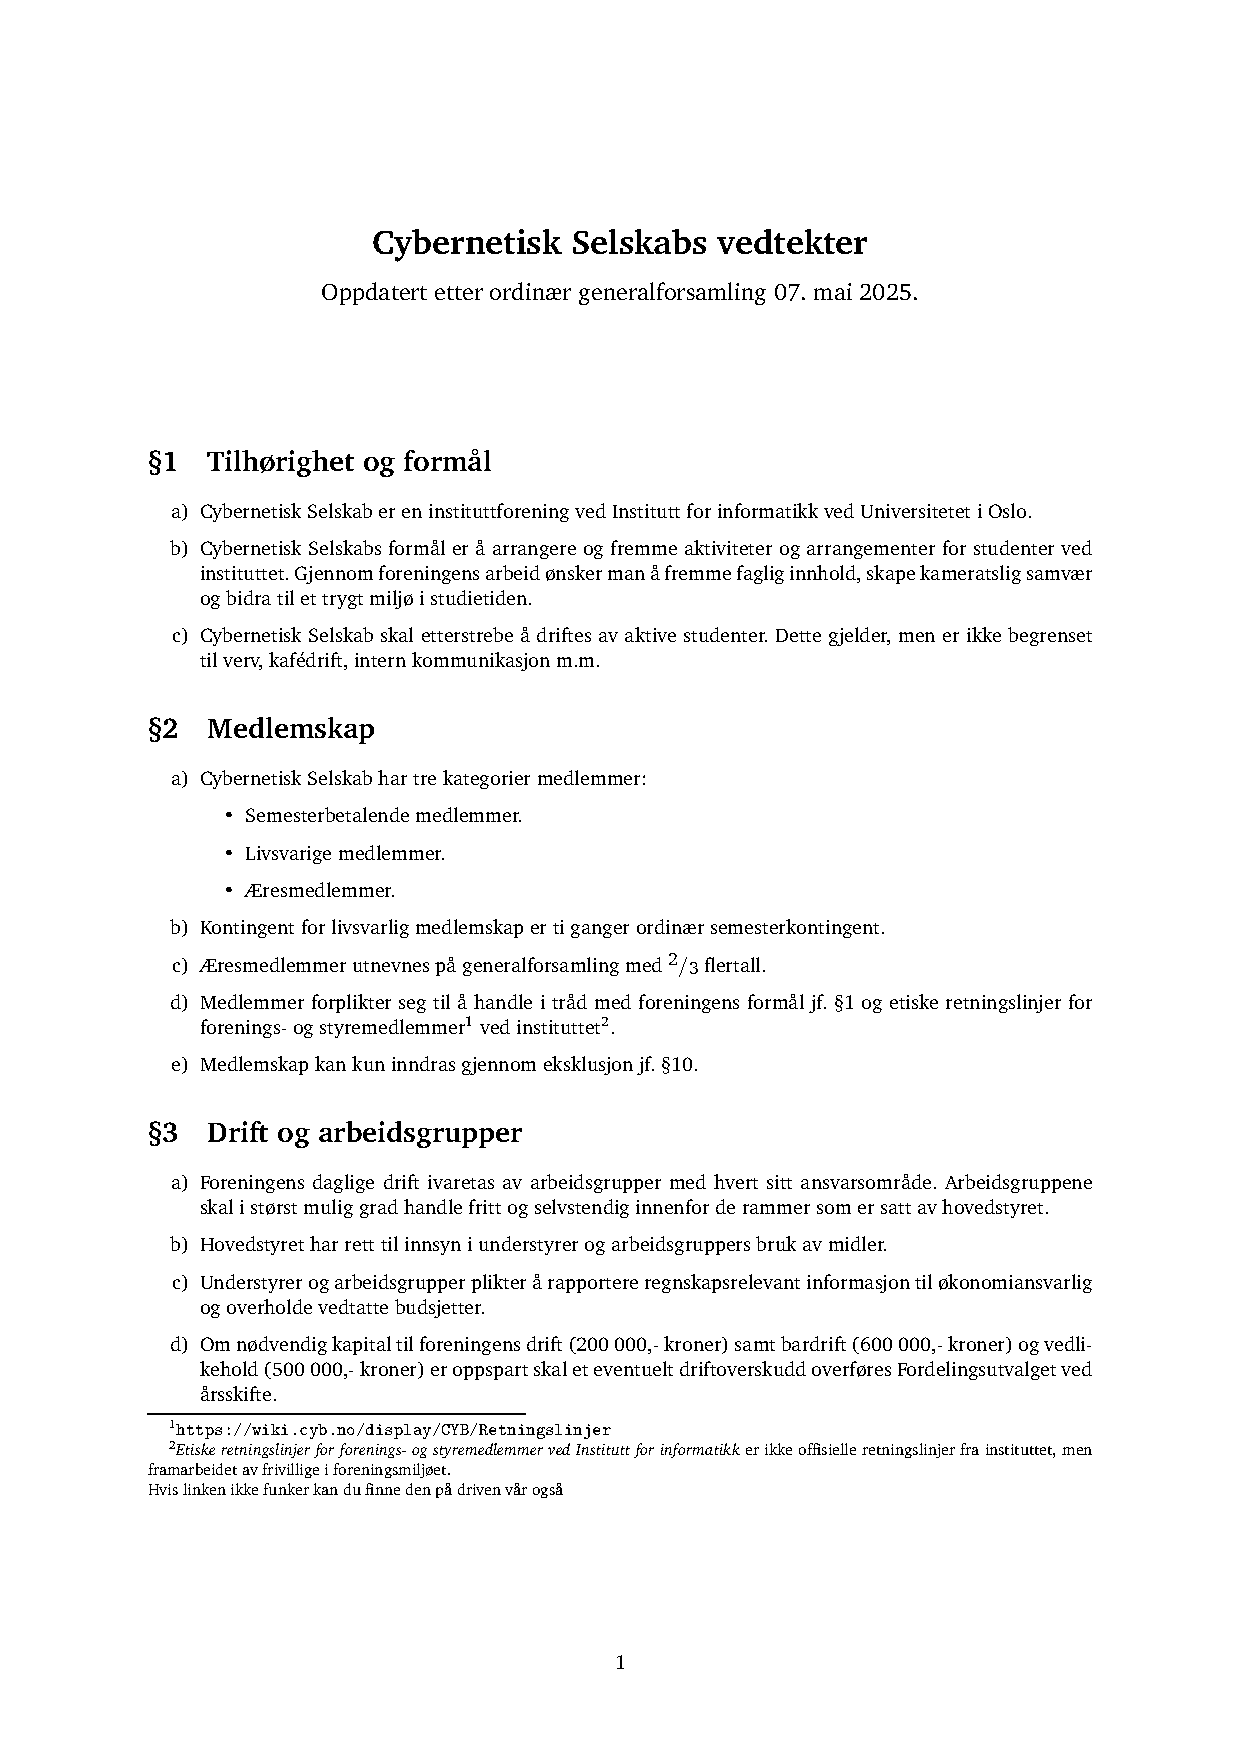
\includepdf[pages=-]{vedtekter.pdf}

\end{document}
